\section{Illustrative Examples for Isotropic Features}\label{sec_special}

%We provide precise explanations to the phenomena of negative transfer in multi-task learning.
%We provide tight bounds on the bias and variance of the multi-task estimator for two tasks.
The results in Section \ref{sec_general} show when multi-task learning outperforms single-task learning for general task covariance matrices and ground truth model parameters.
In particular, the general conditions depend on specific properties of task data such as the covariate shift matrix.
However, the conditions given by the limiting bias and variance of multi-task learning can be difficult to interpret.
The goal of this section is to address this issue.
We interpret the limiting bias and variance equations in an isotropic covariance setting that is described below and a simplified covariate-shifted setting.
We show that three properties of task data affect the performance of multi-task learning as follows.
(i) \textit{Task similarity}: We explain the phenomenon of negative transfer precisely as tasks become more different.
(ii) \textit{Sample ratio}: We further explain a curious phenomenon where increasing the sample ratio between the source and target task helps initially, but hurts eventually.
(iii) \textit{Covariate shift}: Finally, we show that as the sample size of the source task increases, we show that the covariate shift worsens the performance of the multi-task estimator.
%Finally, we provide a extend our results from two tasks to many tasks with the same features.
%We explain from three perspectives, including \textit{task similarity}, \textit{sample size} and \textit{covariate shift}.
%We show how negative transfer occurs by varying task similarity or sample size.
%Then we show that when source task sample size becomes large, covariate shift causes more negative effects.

\smallskip
\noindent\textbf{The isotropic covariance setting.}
	For the two-task case, suppose that the covariates of both tasks have isotropic covariance matrices, that is, $\Sigma_1 = \Sigma_2 = \id$.
%	Each task has sample size $n_1 = \rho_1 \cdot p$ and $n_2 = \rho_2 \cdot p$.
	%And $X_1\in\real^{n_1\times p}, X_2\in\real^{n_2\times p}$ denote the covariates of the two tasks, respectively.
	Assume that for task two, its model parameter, denoted by $\beta_2$, consist of i.i.d. entries with mean zero and variance $\kappa^2$.
	For task one, its model parameter, denoted by $\beta_1$, is equal to $\beta_2$ plus i.i.d. entries with mean $0$ and variance $d^2$.
%	The labels are $Y_i = X_i\beta_i + \varepsilon_i$, where $\e_i$ consists of i.i.d. entries with mean zero and variance $\sigma^2$.
%	For our purpose, it is enough to think of the order of $d$ being $1/\sqrt{p}$ and $pd^2/\sigma^2$ being constant.
%The more precise conditions on the relations between $d^2$, $\sigma^2$ and $\kappa^2$ are given in  \eqref{choiceofpara}.
%	We assume that all the random variables have subexponential decay, while keeping in mind that our results can be applied under weaker moments assumptions as shown in Appendix \ref{sec_maintools}.

%In the isotropic model, we show that as we increase the distance between $\beta_1$ and $\beta_2$ (or $d$), there is a transition from positive transfer to negative transfer in MTL.
%We measure model dissimilarity as $\norm{\beta_1 - \beta_2}^2$, which is the distance between source and target in the isotropic model.
%Figure \ref{fig_model_shift} provides a simulation when $p = 200$.
%{The rest of parameter settings can be found in Appendix \ref{app_synthetic}.}
%Our result below will provide an explanation to this phenomenon.
%Based on Theorem \ref{thm_model_shift}, we derive the transition threshold in the following proposition.
We introduce the following notations.
{\begin{align*}
	\Psi(\beta_1, \beta_2) = {\ex{\bignorm{\beta_1 - \beta_2}^2}} / {\sigma^2},  \quad \Phi(\rho_1, \rho_2) = \frac{(\rho_1 + \rho_2 - 1)^2}{\rho_1 (\rho_1 + \rho_2) (\rho_2 - 1)}.
\end{align*}}


\subsection{Negative Transfer}
It is well-known since the seminal work of Caruana \cite{C97} that how well multi-task learning performs depends on task relatedness.
We formalize this connection in the following simplified setting, where we can perform explicit calculations.
We show that as we increase the distance between $\beta_1$ and $\beta_2$, there is a transition from positive transfer to negative transfer in MTL.
In particular, the bias of MTL increases as the distance between $\beta_1$ and $\beta_2$ increases.
Therefore, while the variance of MTL still reduces compared to STL, if the bias increases more than the amount of variance reduced, we will observe negative transfer.



\begin{proposition}[Task model distance]\label{prop_dist_transition}
	In the isotropic model, suppose that $\rho_1$ and $\rho_2 > 1$.
	Then
	%Whether $\te(\hat{\beta}_t^{\MTL})$ is lower than $\te(\hat{\beta}_t^{\STL})$ is determined by the ratio between $\Psi(\beta_1, \beta_2)$ and $\Phi(\rho_1, \rho_2)$:
	\begin{itemize}
		\item \textbf{Positive transfer:} If $\Psi(\beta_1, \beta_2) < \frac{1}{\nu} \cdot  \Phi(\rho_1, \rho_2)$, then w.h.p. over the randomness of $X_1,X_2$,
			\[ \te(\hat{\beta}_2^{\MTL}) < \te(\hat{\beta}_2^{\STL}). \]
		\item \textbf{Negative transfer:} If $\Psi(\beta_1, \beta_2) > {\nu} \cdot  \Phi(\rho_1, \rho_2)$, then w.h.p. over the randomness of $X_1,X_2$,
			$$\te(\hat{\beta}_2^{\MTL}) > \te(\hat{\beta}_2^{\STL}).$$
	\end{itemize}
	Here {\small$\nu = (1+\oo(1)) \cdot (1 - 1/\sqrt{\rho_1})^{-4}$}.
	Concretely, if $\rho_1 > 40$, then $\nu\in (1,2)$.
\end{proposition}


Proposition \ref{prop_dist_transition} simplifies Theorem \ref{thm_main_informal} in the isotropic model, allowing for a more explicit statement of the bias-variance tradeoff.
Concretely, $\Psi(\beta_1, \beta)$ and $\Phi(\rho_1, \rho_2)$ corresponds to $\Delta_{\bias}$ and $\Delta_{\vari}$, respectively.
%Roughly speaking, the transition threshold scales as $\frac{pd^2}{\sigma^2} - \frac{1}{\rho_1} - \frac{1}{\rho_2}$.
We apply Proposition \ref{prop_dist_transition} to the parameter setting of Figure \ref{fig_model_shift} (the details are left to Appendix \ref{app_synthetic}).
We can see that our result is able to predict positive or negative transfer  accurately and matches the empirical curve.
There are several unexplained observations near the transition threshold $0$, which are caused by the concentration error $\nu$.
%We fix the target task and vary the source task, in particular the parameter $d$ which determines $\norm{\beta_1 - \beta_2}$.
%Figure \ref{fig_model_shift} shows the result.
%We observe that Proposition \ref{prop_dist_transition} explains most of the observations in Figure \ref{fig_model_shift}.
The proof of Proposition \ref{prop_dist_transition} involves two parts.
First, in equation \eqref{eq_te_var}, the positive variance reduction effect scales with $n_1 = \rho_1 p$, the number of source task data points.
Second, we show that the negative effect of model-shift bias scales with $pd^2$, which is the expectation of $\norm{\beta_1 - \beta_2}^2$.
The proof of Proposition \ref{prop_dist_transition} can be found in Appendix \ref{app_proof_31}.
A key part of the analysis shows that $\hat{W}_1 / \hat{W}_2$ is roughly equal to one in the isotropic model,
thus simplifying the general condition in Theorem \ref{thm_main_informal}.

\begin{figure}[!t]
	\begin{subfigure}[b]{0.32\textwidth}
		\centering
		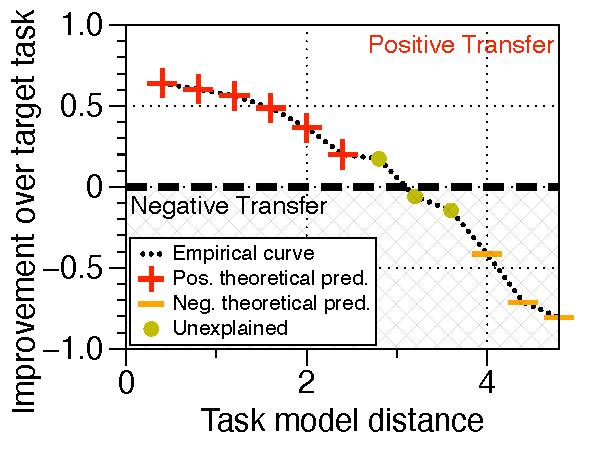
\includegraphics[width=0.98\textwidth]{figures/model_shift_phase_transition.pdf}
		\caption{Task similarity}
		\label{fig_model_shift}
	\end{subfigure}\hfill
	\begin{subfigure}[b]{0.32\textwidth}
		\centering
		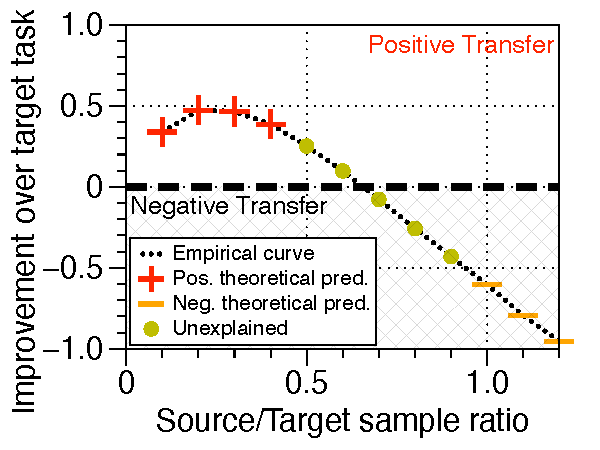
\includegraphics[width=0.98\textwidth]{figures/datapoints_phase_transition.pdf}
		\caption{Sample size}
		\label{fig_size}
	\end{subfigure}\hfill
	\begin{subfigure}[b]{0.32\textwidth}
		\centering
		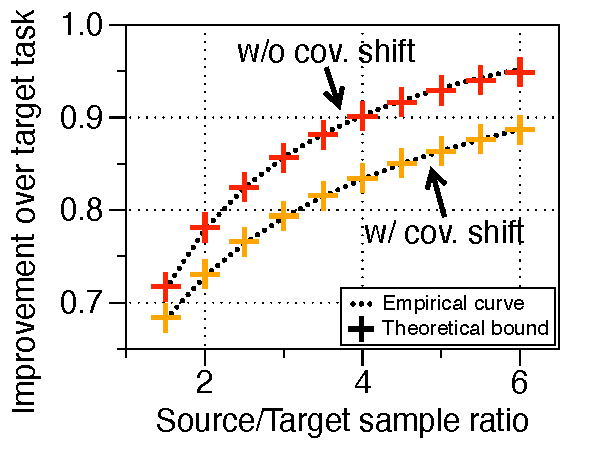
\includegraphics[width=0.98\textwidth]{figures/complementary.pdf}
		\caption{Covariate shift}
		\label{fig_covariate}
	\end{subfigure}
	\caption{%Three takeaways of our theory in Section \ref{sec_insight}.
	We observe a transition from positive to negative transfer as (a) \textit{task model distance} increases and (b) source/target \textit{sample ratio} increases.
	For the special case of having the same task model, we observe in (c) that as source/target \textit{sample ratio} increases, having \textit{covariate shift} worsens the performance of MTL.
	The $y$-axis measures the loss of STL minus MTL.}
	\label{fig_model_shift_phasetrans}
\end{figure}

%\subsection{Sample Ratio}\label{sec_data_size}

In classical Rademacher or VC based theory of multi-task learning, the generalization bounds are usually presented for settings where the sample sizes are equal for all tasks \cite{B00,M06,MPR16}.
%More generally, such results are still applicable when all task data are being added simultaneously.
On the other hand, uneven sample sizes between different tasks (or even dominating tasks) have been empirically observed as a cause of negative transfer \cite{YKGLHF20}.
For such settings, we have also observed that adding more labeled data from one task does not always help.
%On the other hand, we have observed that adding more labeled data does not always improve performance in multi-task learning.
In the isotropic model, we consider what happens if we vary the source task sample size.
Our theory accurately predicts a curious phenomenon, where increasing the sample size of the source task results in negative transfer!
Figure \ref{fig_size} provides a simulation result for such a setting.
We observe that as $n_1 / n_2$ increases, there is a transition from positive to negative transfer.

\begin{proposition}[Source/target sample ratio]\label{prop_data_size}
	In the isotropic model, suppose that $\rho_1 > 40$ and $\rho_2 > 110$ are fixed constants, and $\Psi(\beta_1, \beta_2) > 2/(\rho_2 - 1)$.
	Then we have that
	\begin{itemize}
		\item \textbf{Positive transfer:} If $\frac{n_1}{n_2} = \frac{\rho_1}{\rho_2} < \frac{1}{\nu} \cdot \frac{1 - 2\rho_2^{-1}}{\Psi(\beta_1, \beta_2) (\rho_2 - 1) - \nu^{-1}}$, then w.h.p. $$\te(\hat{\beta}_2^{\MTL}) < \te(\hat{\beta}_2^{\STL}).$$
		\item \textbf{Negative transfer:} If $\frac{n_1}{n_2} = \frac{\rho_1}{\rho_2} > {\nu} \cdot \frac{1 - 2\rho_2^{-1}}{\Psi(\beta_1, \beta_2) (\rho_2 - 3/2) - \nu}$, then w.h.p. $$\te(\hat{\beta}_2^{\MTL}) > \te(\hat{\beta}_2^{\STL}).$$
	\end{itemize}
\end{proposition}
Proposition \ref{prop_data_size} describes the bias-variance tradeoff in terms of the sample ratio $\rho_1 / \rho_2$.
We apply the result to the setting of Figure \ref{fig_size} (described in Appendix \ref{app_synthetic}).
There are several unexplained observations near $y = 0$ caused by $\nu$.
The proof of Proposition \ref{prop_data_size} can be found in Appendix \ref{app_proof_32}.

\subsection{Covariate Shift} \label{sec_covshift}
So far we have considered the isotropic model where $\Sigma_1 = \Sigma_2$.
This setting is relevant for settings where different tasks share the same input features such as multi-class image classification.
In general, the covariance matrices of the two tasks may be different such as in text classification.
In this part, we consider what happens when $\Sigma_1 \neq \Sigma_2$.
We show that when $n_1 / n_2$ is large, MTL with covariate shift can be suboptimal compared to MTL without covariate shift.

\noindent\textit{Example.}
	We measure covariate shift by $M = \Sigma_1^{1/2} \Sigma_2^{-1/2}$ similar to Theorem \ref{thm_main_informal}.
	We assume that the two tasks have the same ground truth model parameters, that is, $\beta_1 = \beta_2$ and $\Psi(\beta_1, \beta_2) = 0$.
	We compare two cases: (i) when $M = \id_{p\times p}$; (ii) when $M$ has $p/2$ singular values that are equal to $\lambda$ and $p/2$ singular values that are equal to $1 / \lambda$.
	Hence, $\lambda$ measures the severity of the covariate shift.
	Figure \ref{fig_covariate} shows a simulation of this setting by varying $\lambda$.
	We observe that as source/target sample ratio increases, the performance gap between the two cases increases.

%By applying Lemma \ref{lem_cov_shift_informal}, we find that when $n_1 / n_2$ is large, having no covariate shift is the optimal choice provided that the determinant of $M^{\top}M$ is bounded.
We compare different choices of $M$ that belong to the following bounded set.
Let $\lambda_i$ be the $i$-th singular value of $M$.
Let $\mu_{\min} < \mu < \mu_{\max}$ be fixed values that do not grow with $p$.
{\begin{align*}
		\cS_{\mu}\define\bigset{M \left| \prod_{i=1}^p \lambda_i \le \mu^p, \mu_{\min} \le \lambda_i\le \mu_{\max}, \text{ for all } 1\le i\le p\right.},
\end{align*}}
%	We assume that $\beta_1$ and $\beta_2$ are generated following the isotropic model with $d = 0$.
\begin{proposition}[Covariate shift]\label{prop_covariate}
	For the setting of the example above, assume that $\beta_1 = \beta_2$, $\rho_1$ and $\rho_2$ are both greater than one.
	Let $g(M)$ denote the prediction loss of $\hat{\beta}_t^{\MTL}$ when $M = \Sigma_1^{1/2}\Sigma_2^{-1/2} \in\cS_{\mu}$.
	We have that
		\[ g(\mu\id) \le \bigbrace{1+ \bigo{{\rho_2}/{\rho_1}  }} \min_{M\in\cS_{\mu}} g(M). \]
\end{proposition}
Proposition \ref{prop_covariate} shows that when the sample ratio is large, having no covariate shift gives the optimal performance for multi-task learning.
The proof of Proposition \ref{prop_covariate} can be found in Appendix \ref{app_proof_33}.
%Proposition \ref{prop_covariate} implies that when $\rho_1\gg \rho_2$, having no covariate shift is the optimal choice for choosing the source task.
%This provides evidence that covariate shift is unfavorable when there are many source task datapoints,

%\todo{} To complement the result, we show an example when the statement is not true if $n_1 \le n_2$.

%We ask: is it better to have $M$ as being close to identity, or should $M$ involve varying levels of singular values?
%Understanding this question has implications for applying normalization methods in multi-task learning \cite{LV19,CBLR18,YKGLHF20}.
%We show that if $n_1$ is much larger than $n_2$, then the optimal $M$ matrix should be proportional to identity, under certain assumptions on its range of singular values (to be formulated in Proposition \ref{prop_covariate}).
%On the other hand, if $n_1$ is comparable or even smaller than $n_2$, we show an example where having ``complementary'' covariance matrices is better performing than having the same covariance matrices.



\subsection{Data Efficiency}

observed in Taskonomy \cite{ZSSGM18}.




\section{Main Results for General Features}\label{sec_general}

%\begin{proposition}[Bias-variance tradeoff]
%	Variance always reduces and bias always increases.
%\end{proposition}
In this section, we compare the prediction loss of the multi-task learning estimator to that of the single-task learning estimator.
First, we consider the two-task case.
We provide precise asymptotics of the bias and variance of the multi-task learning estimator.
We apply recent developments from the random matrix theory literature to characterize the bias and variance.
The results scale with key properties of task data such as sample size and covariance shift, and allow us to study the performance of multi-task learning by varying these properties (Section \ref{sec_special}).
Second, we consider the multiple-task case where all tasks have the same features but different labels.
We extend the bias-variance decomposition of the two-task case to this setting and show qualitatively similar results.
%For the single-task learning estimator, there are well-known results that relate its prediction loss to sample size and noise variance.

%We focus on the high-dimensional linear regression setting \cite{}






\paragraph{Same covariates.}
%A well-known result in the high-dimensional linear regression setting states that $\tr[(X_2^{\top}X_2)^{-1}\Sigma_2]$ is concentrated around $1 / (\rho_2 - 1)$ (e.g. Chapter 6 of \cite{S07}), which scales with the sample size of the target task.
%Our main technical contribution is to extend this result to two tasks.
%We show how the variance of the multi-task estimator scales with sample size and covariate shift in the following result.
Next, we describe our result for the multiple-task case where all tasks have the same covariates, that is, $X_i = X$, $n_i = n$, and $\Sigma_i = \Sigma$ for all $i = 1, \dots, t$.
This setting is prevalent in applications of multi-task learning to image classification, where there are multiple prediction labels/tasks for every image \cite{chexnet17,EA20}.
Similar to the two-task case, we consider an arbitrary local minimum $B, W_1, \dots, W_2$ of the optimization objective.
We extend the bias-variance decomposition from the two-task case to the multiple-task case.
Let $\cal W = [W_1, W_2, \dots, W_t] \in \real^{r\times t}$ be a matrix that contains all the parameters of the output layers.
We observe that the expected prediction loss of $\hat{\beta}_t^{\MTL}$ conditional on $X$ consists of a bias and a variance equation as follows
\begin{align}
	\exarg{\varepsilon_1, \dots, \varepsilon_t}{L(\hat{\beta}_t^{\MTL}) \mid X}
	=& \bignorm{\Sigma^{1/2} \bigbrace{B^{\star} \cW^{\top} (\cW \cW^{\top})^{-1} W_t - \beta_t}}^2 \label{eq_bias_multiple} \\
	&+ \sigma^2 \cdot (W_t^{\top} (\cW \cW^{\top})^{-1} W_t) \cdot \bigtr{\Sigma (X^{\top} X)^{-1}} \label{eq_var_multiple}
\end{align}
One can see that equation \eqref{eq_bias_multiple} is the bias of the multi-task learning estimator and equation \eqref{eq_var_multiple} is its variance.
Compared to the prediction loss of single-task learning (cf. equation \eqref{eq_var_stl}), we observe that the variance equation \eqref{eq_var_multiple} is always smaller because $W_t^{\top} (\cW \cW^{\top})^{-1} W_t \le 1$.
On the other hand, the bias equation \eqref{eq_bias_multiple} is always larger because of the difference between the task models.

Our main result for the multiple-task case provides generalization bounds that relate the empirical bias and variance of multi-task learning to the sample size $n$ and the distance between task models.
Before stating the result, we define the following notations.
Let $B^\star := [{\beta}_1,{\beta}_2,\dots,{\beta}_{t}] \in \real^{p\times t}$ denote the ground truth model parameters.
Let $U_r U_r^{\top}$ denote the best rank-$r$ subspace approximation of $(B^{\star})^\top\Sigma B^{\star}$, that is,
\[ U_r \define \argmin_{X\in\real^{t\times r} : X^{\top} X = \id_{r\times r}} \inner{X X^{\top}} {B^{\star} \Sigma B^{\star}}. \]
For $i = 1,\dots, t$, let $v_i \in\real^r$ denote the $i$-th row of $U_r$.

\begin{theorem}[Multiple-task case with the same covariates]\label{thm_many_tasks}
%Suppose $X=Z\Sigma^{1/2}\in \R^{n\times p}$ satisfy Assumption \ref{assm_secA1} with $\rho:=n/p>1$ being some fixed constant. Consider data models  $Y_i = X\beta_i + \varepsilon_i$, $i=1,2,\cdots, t$, where $\e_i\in \R^{n}$ are random vectors with i.i.d. entries with mean zero, variance $\sigma^2$ and all moments as in \eqref{assmAhigh}. Moreover, assume that $X$, $\beta_i$ and $\e_i$ are all independent of each other.
	%Let $n = c \cdot p$.
	%Let $X\in\real^{n\times p}$ and $Y_i = X\beta_i + \varepsilon_i$, for $i = 1,\dots,k$.
%	Consider $t$ data models $Y_i = X\beta_i + \varepsilon_i$, $i=1,2,\cdots, t$, where $X$ has covariance matrix $\Sigma$, and the entries of $\e_i$ are i.i.d. with mean zero and variance $\sigma^2$.
	%that satisfy Assumption \ref{assm_secA2} in the appendix.
	Consider the multiple-task case where all tasks have the same covariates.
	Assume that $\lambda_{\min}({B^{\star}}^\top\Sigma B^{\star})\gtrsim \sigma^2$.
	Let $\delta$ be any fixed value such that $\delta \le \oo \left( \|B^\star\|^2 + \sigma^2\right)$.
	Then, the following is true:
	\begin{itemize}
		\item \textbf{Positive transfer:} If $\left(1 - \norm{v_t}^2 \right)\frac{\sigma^2}{\rho - 1} - \norm{\Sigma^{1/2} (B^{\star} U_r v_t - \beta_t)}^2 > \delta$, then w.h.p over the randomness of $X, \varepsilon_1, \dots, \varepsilon_t$, we have that
		 \[ \te(\hat{\beta}_t^{\MTL}) < \te(\hat{\beta}_t^{\STL}). \]
		\item \textbf{Negative transfer:} If $\left(1 - \norm{v_t}^2\right)\frac{\sigma^2}{\rho - 1} - \norm{\Sigma^{1/2}(B^{\star} U_r v_t - \beta_t)}^2 < -\delta$, then w.h.p. over the randomness of $X, \varepsilon_1, \dots, \varepsilon_t$, we have that
		\[ \te(\hat{\beta}_t^{\MTL}) > \te(\hat{\beta}_t^{\STL}). \]
	\end{itemize}
\end{theorem}
Theorem \ref{thm_many_tasks} provides a sharp analysis of the bias-variance tradeoff in the multiple-task case.
As shown in the proof of Theorem \ref{thm_many_tasks}, the equation $(1 - \norm{v_t}^2)\frac {\sigma^2}{\rho - 1}$ is the amount of variance reduced using multi-task learning and $\norm{\Sigma (B^{\star} U_r v_t - \beta_t)}$ is the bias.
The proof of \ref{thm_many_tasks} can be found in Section \ref{app_proof_many_tasks}.





\paragraph{Different covariates: the two-task case.}
As mentioned in Section \ref{sec_prelim}, the optimization objective \eqref{eq_mtl} is non-convex in general.
Therefore, we consider an arbitrary local minimum $B, W_1, W_2$, in particular when $B = \hat{B}(W_1, W_2)$ satisfies the local optimality condition.
We derive deterministic conditions to compare the prediction loss of the local minimum to single-task learning.
Our key insight is a bias-variance decomposition of the expected prediction loss of $\hat{\beta}_2^{\MTL} = \hat{B} W_2$ as follows
\begin{align}
	\exarg{\epsilon_1, \epsilon_2}{L(\hat{\beta}_2^{\MTL}) \mid X_1, X_2}
	=&~ \frac{W_1^2}{W_2^2} \bignorm{\Sigma_2^{1/2}(\frac{W_1^2}{W_2^2} X_1^{\top}X_1 + X_2^{\top}X_2)^{-1} X_1^{\top}X_1 (\beta_1 - \frac{W_1}{W_2} \beta_2)}^2 \label{eq_bias_2task} \\
			&+~  \sigma^2\cdot \bigtr{\Sigma_2(\frac{W_1^2}{W_2^2} X_1^{\top}X_1 + X_2^{\top}X_2)^{-1} }. \label{eq_var_2task}
\end{align}
See Section \ref{app_proof_main_thm} for its derivation.
Equation \eqref{eq_bias_2task} is the bias of $\hat{\beta}_t^{\MTL}$ and
equation \eqref{eq_var_2task} is the variance of $\hat{\beta}_t^{\MTL}$.
%minus the variance of $\hat{\beta}_t^{\STL}$, which is always negative.
Comparing the above to single-task learning, that is,
\begin{align}
	\exarg{\epsilon_2}{L(\hat{\beta}_2^{\STL}) \mid X_2} = \sigma^2 \cdot \bigtr{\Sigma_2 (X_2^{\top} X_2)^{-1}}, \label{eq_var_stl}
\end{align}
we observe that while the bias of $\hat{\beta}_2^{\MTL}$ is always larger than that of $\hat{\beta}_2^{\STL}$, which is zero, the variance of $\hat{\beta}_2^{\MTL}$ is always lower than that of $\hat{\beta}_2^{\STL}$.\footnote{To see why this is true, we apply the Woodbury matrix identity over equation \eqref{eq_var_2task} and use the fact that for the product of two PSD matrices, its trace is always nonnegative.}
In other words, training both tasks together helps predict the target task by reducing variance while incurring a bias.
Therefore, whether multi-task learning outperforms single-task learning is determined by the bias-variance decomposition!


Based on the above intuition, in the following we develop generalization bounds that relate the bias and variance of multi-task learning to the sample sizes and the covariance matrices of both tasks.
We introduce a key quantity $M = \Sigma_1^{1/2}\Sigma_2^{-1/2}$ that captures the covariate shift between task $1$ and task $2$.

%We now state our main result for two tasks with both covariate and model shift. It shows that the information transfer is determined by two deterministic quantities $\Delta_{\bias}$ and $\Delta_{\vari}$, which give the change of model shift bias and the change of variance, respectively. The exact forms of $\Delta_{\bias}$ and $\Delta_{\vari}$ will be given in Lemma \ref{thm_model_shift}.

\begin{theorem}[Two-task case]\label{thm_main_informal}
	%For the setting of two tasks, let $\delta > 0$ be a fixed error margin, $\rho_2 > 1$ and $\rho_1 \gtrsim \delta^{-2}\cdot \lambda_{\min}(M)^{-4} \norm{\Sigma_1} \max(\norm{\beta_1}^2, \norm{\beta_2}^2)$.
	For the setting of two tasks, let $C$ be a fixed constant and let $\delta = \frac{ C\cdot \max(\norm{\beta_1}, \norm{\beta_2}) \cdot \sqrt{\norm{\Sigma_1}} } {\lambda_{\min}^2(M)) }$.
	Let $B, W_1, W_2$ be any local minimum of equation \eqref{eq_mtl}.
 	There exist two deterministic functions $\Delta_{\bias}$ and $\Delta_{\vari}$ that only depend on scaled model distance $\beta_1 - \frac{W_1}{W_2} \beta_2$, sample sizes $n_1 = \rho_1 \cdot p, n_2 = \rho_2 \cdot p$, and covariate shift matrix $M$ such that
	\begin{enumerate}
		\item[a)] \textbf{Positive transfer:} If $\Delta_{\bias} < \Delta_{\vari} -  \frac{\delta}{\sqrt{\rho_1}} $, then w.h.p. over the randomness of $X_1, X_2, \varepsilon_1, \varepsilon_2$, we have
			\[ \te(\hat{\beta}_2^{\MTL}) < \te(\hat{\beta}_2^{\STL}).  \]
		\item[b)] \textbf{Negative transfer:} If $\Delta_{\bias} > \Delta_{\vari} + \frac{\delta}{\sqrt{\rho_1}}$, then w.h.p. over the randomness of $X_1, X_2, \varepsilon_1, \varepsilon_2$, we have
			\[ \te(\hat{\beta}_2^{\MTL}) > \te(\hat{\beta}_2^{\STL}). \]
	\end{enumerate}
\end{theorem}
In words, the above result shows that a deterministic function $\Delta_{\bias} - \Delta_{\vari}$ determines whether the prediction loss of the empirical multi-task learning estimator is lower than that of single-task learning, up to an error that scales as $\delta / \sqrt{\rho_1}$.
We make several remarks about Theorem \ref{thm_main_informal}.
First, as the amount of data from the source task increases, we get more accurate predictions  since the error scales down.
This applies to many practical settings where collecting labeled data for the target task is expensive and auxillary (source) task data is easier to obtain.
%Theorem \ref{thm_main_informal} applies to settings where large amounts of source task data are available but the target sample size is small.
%For such settings, we obtain a sharp transition from positive transfer to negative transfer determined by $\Delta_{\bias} - \Delta_{\vari}$.
%determined by the covariate shift matrix and the model shift.
%The bounds get tighter and tighter as $\rho_1$ increases.
Second, the deterministic function $\Delta_{\bias} - \Delta_{\vari}$ depends on the three task properties that we care about and the precise form can be found in Section \ref{sec_proof_general}.
Finally, later on in Section \ref{sec_special}, we will study how varying each task property affects the performance of multi-task learning in depth.
%While the general form of these functions can be complex (as are previous generalization bounds for MTL), they admit interpretable forms for simplified settings.

%\textbf{Proof overview.}\todo{}
%Theorem \ref{lem_cov_shift_informal} extends a well-known result for the single-task setting when $X_1, \rho_1, a_1$ are all equal to zero \cite{S07}.
%Applying Theorem \ref{lem_cov_shift_informal} to \eqref{eq_te_var}, we can calculate the amount of reduced variance compared to STL, which is given asymptotically by $\Delta_{\vari}$.
%For the bias term in equation \eqref{eq_te_model_shift}, we apply the approximate isometry property to $X_1^{\top}X_1$, which is close to $n_1^2\Sigma_1$. This results in the error term $\delta$, which scales as $(1 + 1/\sqrt{\rho_1})^4-1$.
%Then, we apply a similar identity to Theorem \ref{lem_cov_shift_informal} for bounding the bias term, noting that the derivative of $R(z)$ with respect to $z$ can be approximated by $R_\infty'(z)$.
%This estimates the negative effect given by $\Delta_{\bias}$. %, which will be used to estimate the first term on the right hand side of \eqref{eq_te_model_shift}.
%During this process, we will get the $\Delta_{\bias}$ term up to an error $\delta$ depending on $\rho_1$.
%The proof of Theorem \ref{thm_main_informal} is presented in Appendix \ref{app_proof_main_thm} and the proof of Lemma \ref{lem_cov_shift_informal} is in Appendix \ref{sec_maintools}.
%
%
%
%The formal statement is stated in Theorem \ref{thm_many_tasks} and its proof can be found in Appendix \ref{app_proof_many_tasks}.
%The technical crux of our approach is to derive the asymptotic limit of $\te(\hat{\beta}_t^{\MTL})$ in the high-dimensional setting, when $p$ approaches infinity.
%We derive a precise limit of $\bigtr{(X_1^{\top}X_1 + X_2^{\top}X_2)^{-1}\Sigma_2}$, which is a deterministic function that only depends on $\Sigma_1, \Sigma_2$ and $n_1/p, n_2/p$ (see Lemma \ref{lem_cov_shift} in Appendix \ref{app_proof_main} for the result).
%Based on the result, we show how to determine positive versus negative transfer as follows.
%, where $\lambda_{\min}(M)$ is the smallest singular value of $M_1$

\iffalse
Next, we derive a closed-form solution of the multi-task learning estimator for the case of two tasks.
From \cite{WZR20}, we know that we need to explicitly restrict the output dimension $r$ of $B$ so that there is transfer between the two tasks.
Hence for the case of two tasks, we consider the setting where $r=1$.
For simplicity of notations, we shall denote $(X_i^{tr},Y_i^{tr})$ and $(X_i^{val},Y_i^{val})$ as $(X_i,Y_i)$ and  $(\wt X_i,\wt Y_i)$, respectively. Then equation \eqref{eq_mtl} simplifies to
\begin{align}\label{eq_mtl_2task}
	f(B; w_1, w_2) = \bignorm{X_1 B w_1 - Y_1}^2 + \bignorm{X_2 B w_2 - Y_2}^2,
\end{align}
where $B\in\real^p$ and $w_1, w_2$ are both real numbers. To solve the above problem, suppose that $w_1, w_2$ are fixed, by local optimality, we find the optimal $B$ as
\begin{align}
	& \hat{B}(w_1, w_2) = (w_1^2 X_1^{\top}X_1 + w_2^2 X_2^{\top}X_2)^{-1} (w_1 X_1^{\top}Y_1 + w_2 X_2^{\top}Y_2) \label{hatB}\\
	&= \frac{1}{w_2} \left( \frac{w_1^2}{w_2^2}  X_1^{\top}X_1 + X_2^{\top}X_2\right)^{-1} \left(\frac{w_1}{w_2} X_1^{\top}Y_1 + X_2^{\top}Y_2\right) \nonumber\\
	&= \frac{1}{w_2}\left[\beta_2 + \left(\frac{w_1^2}{w_2^2} X_1^{\top}X_1 + X_2^{\top}X_2\right)^{-1}\bigbrace{X_1^{\top}X_1\left(\frac{w_1}{w_2}\beta_1 - \frac{w_1^2}{w_2^2} \beta_2\right) + \left(\frac{w_1}{w_2} X_1^{\top}\varepsilon_1 + X_2^{\top}\varepsilon_2\right)}\right]. \nonumber
\end{align}
As a remark, when $w_1 = w_2 = 1$, we obtain linear regression.
If $\beta_1$ is a scaling of $\beta_2$, then  $w_1, w_2$ can be scaled accordingly to fix both tasks more accurately than linear regression.

%For the discussions below, we assume that the entries of $\e_1$ and $\e_2$ all have the same variance $\sigma^2$. This holds for most parts of our discussion, except in Proposition \ref{prop_var_transition}. We will derive different expressions for the validation loss and the test error

Next we consider $N_i$ independent samples of the training set $\{(\wt x_k^{(i)},\wt y_k^{(i)}): 1\le k \le N_i\}$ from task-$i$, $i=1,2$. With these sample, we form the random matrices $\wt X_i \in \R^{N_i\times p}$ and $\wt Y_i\in \R^{N_i}$, $i=1,2,$ whose row vectors are given by $\wt x_k^{(i)}$ and $\wt y_k^{(i)}$. We assume that $N_1$ and $N_2$ satisfy $N_1/N_2=n_1/n_2$ and $N_i \ge n_i^{1-\e_0}$ for some constant $\e_0>0$. Then we write the validation loss in \eqref{eq_mtl_eval} as
\begin{align}\label{eq_mtl_2tasktilde}
	g(w_1,w_2) = \bignorm{\wt X_1 \hat B w_1 - \wt Y_1}^2 + \bignorm{\wt X_2 \hat B w_2 - \wt Y_2}^2.
\end{align}
Inserting \eqref{hatB} into \eqref{eq_mtl_2tasktilde}, one can see that the optimal solution of $g$ only depends on the ratio $v:=w_1/w_2$.
Hence we overload the notation by writing $g(v)$ in the following discussion.
The expectation of $g(v)$ can be written as follows.
\begin{align}
		\val(v) \define& \exarg{\varepsilon_1,\e_2} {\sum_{i=1}^2 \left\|\Sigma_i^{1/2}( \hat B w_i - \beta_i) \right\|^2} \nonumber\\
	=&  N_1 \cdot \bignorm{\Sigma_1^{1/2}\left(v^2 X_1^{\top}X_1 + X_2^{\top}X_2\right)^{-1}X_2^{\top}X_2\left (\beta_1 - v\beta_2\right)}^2 \nonumber \\
	&+ N_2 \cdot v^2\bignorm{\Sigma_2^{1/2}\left(v^2 X_1^{\top}X_1 + X_2^{\top}X_2\right)^{-1}X_1^{\top}X_1\left(\beta_1 - v\beta_2\right)}^2 \nonumber \\
		&+ N_1   \cdot v^2 \bigtr{\Sigma_1\left(v^2 X_1^{\top}X_1 + X_2^{\top}X_2\right)^{-2} \left(\sigma_1^2 \cdot v^2X_1^{\top}X_1 + \sigma_2^2 \cdot X_2^{\top}X_2\right)} \nonumber \\
		&+ N_2  \cdot \bigtr{\Sigma_2\left(v^2 X_1^{\top}X_1 + X_2^{\top}X_2\right)^{-2} \left(\sigma_1^2 \cdot v^2  X_1^{\top}X_1 + \sigma_2^2  \cdot X_2^{\top}X_2\right)}. \label{revise_eq_val_mtl}
\end{align}

{\color{red}\begin{align*}
			& f(W_1, W_2) = \bignorm{X_1 \hat B w_1 - Y_1}^2 + \bignorm{X_2 \hat B w_2 - Y_2}^2\\
			& =\bignorm{X_1\left( v^2 X_1^{\top}X_1 + X_2^{\top}X_2\right)^{-1} \left(v^2 X_1^{\top}Y_1 + vX_2^{\top}Y_2\right) - Y_1}^2 \\
			&+ \bignorm{X_2 \left( v^2 X_1^{\top}X_1 + X_2^{\top}X_2\right)^{-1} \left(vX_1^{\top}Y_1 + X_2^{\top}Y_2\right) - Y_2}^2 \\
			& =\bignorm{X_1\left( v^2 X_1^{\top}X_1 + X_2^{\top}X_2\right)^{-1} \left(v^2 X_1^{\top}\e_1 + vX_2^{\top}\e_2\right) - \e_1 + X_1\left( v^2 X_1^{\top}X_1 + X_2^{\top}X_2\right)^{-1}  X_2^{\top}X_2(v\beta_2-\beta_1) }^2 \\
			&+ \bignorm{X_2 \left( v^2 X_1^{\top}X_1 + X_2^{\top}X_2\right)^{-1} \left(vX_1^{\top}\e_1 + X_2^{\top}\e_2\right) - \e_2 + vX_2 \left( v^2 X_1^{\top}X_1 + X_2^{\top}X_2\right)^{-1}  X_1^{\top}X_1(\beta_1-v\beta_2) }^2 \\
			&=\val(v)\cdot \left( 1+\OO(p^{-1/2\e})\right) \quad \text{w.h.p.},
		\end{align*}
		where
		\begin{align*}
		\val(v)&=\bignorm{X_1\left( v^2 X_1^{\top}X_1 + X_2^{\top}X_2\right)^{-1}  X_2^{\top}X_2(v\beta_2-\beta_1) }^2 \\
			&+ v^2\bignorm{X_2 \left( v^2 X_1^{\top}X_1 + X_2^{\top}X_2\right)^{-1}  X_1^{\top}X_1(\beta_1-v\beta_2) }^2 \\
			&+\sigma^2 \tr\left(v^2 X_1\left( v^2 X_1^{\top}X_1 + X_2^{\top}X_2\right)^{-1}   X_1^{\top} -\id\right)^2 \\
			&+\sigma^2 \tr\left(v^2 X_1\left( v^2 X_1^{\top}X_1 + X_2^{\top}X_2\right)^{-1}X_2^{\top}X_2 \left( v^2 X_1^{\top}X_1 + X_2^{\top}X_2\right)^{-1} X_1^\top\right)\\
			&+\sigma^2 \tr\left(X_2 \left( v^2 X_1^{\top}X_1 + X_2^{\top}X_2\right)^{-1} X_2^{\top} -\id\right)^2 \\
			&+\sigma^2 \tr\left(v^2 X_2\left( v^2 X_1^{\top}X_1 + X_2^{\top}X_2\right)^{-1}X_1^{\top}X_1 \left( v^2 X_1^{\top}X_1 + X_2^{\top}X_2\right)^{-1} X_2^\top\right)\\
			&=\bignorm{X_1\left( v^2 X_1^{\top}X_1 + X_2^{\top}X_2\right)^{-1}  X_2^{\top}X_2(v\beta_2-\beta_1) }^2 \\
			&+ v^2\bignorm{X_2 \left( v^2 X_1^{\top}X_1 + X_2^{\top}X_2\right)^{-1}  X_1^{\top}X_1(\beta_1-v\beta_2) }^2 +(n_1+n_2-p)\sigma^2.
		\end{align*}
	}





Hence to minimize $g(v)$, it suffices to minimize $\val(v)$ over $v$.
Let $\hat v=\hat{w_1}/\hat{w_2}$ be the global minimizer of $g(v)$.
Now we can define the multi-task learning estimator for the target task as
	\[ \hat{\beta}_2^{\MTL} = \hat{w}_{2}\hat{B}(\hat{w}_1, \hat{w}_2) .\]
%	where $t=2$ since we are considering the two task case, and it also stands for the ``target task".
%The intuition for deriving $\hat{\beta}_2^{\MTL}$ is akin to performing multi-task training in practice.
%Let $\hat{v} = \hat{w_1} / \hat{w_2}$ for the simplicity of notation.
The prediction loss of using $\hat{\beta}_2^{\MTL}$ for the target task is
\begin{align}
	\te(\hat{\beta}_2^{\MTL}) =&~ \hat{v}^2 \bignorm{\Sigma_2^{1/2}(\hat{v}^2 X_1^{\top}X_1 + X_2^{\top}X_2)^{-1} X_1^{\top}X_1 (\beta_1 - \hat{v} \beta_2)}^2 \nonumber \\
			&+~  \bigtr{\Sigma_2(\hat{v}^2 X_1^{\top}X_1 + X_2^{\top}X_2)^{-2}\left(\sigma_1^2 \cdot \hat v^2  X_1^{\top}X_1 + \sigma_2^2  \cdot X_2^{\top}X_2\right) }, \label{eq_te_mtl_2task}
\end{align}
which only depends on $\hat v$, the sample covariance matrices, and $\beta_1,\beta_2$.
\fi

%\begin{lemma}[Variance bound]\label{lem_cov_shift_informal}
%	In the setting of two tasks,
%	let $n_1 = \rho_1 \cdot p$ and $n_2 = \rho_2 \cdot$ be the sample size of the two tasks.
%	Let $\lambda_1, \dots, \lambda_p$ be the singular values of the covariate shift matrix $\Sigma_1^{1/2}\Sigma_2^{-1/2}$ in decreasing order.
%	%let $n_1 = \rho_1 \cdot p$ and $n_2 = \rho_2 \cdot p$ denote the sample sizes of each task.
%	%Let $\Sigma_1$ and $\Sigma_2$ denote the covariance matrix of each task.
%	With high probability, the variance of the multi-task estimator $\hat{\beta}_t^{\MTL}$ equals
%	%let $M = \Sigma_1^{1/2}\Sigma_2^{-1/2}$ and $\lambda_1, \lambda_2, \dots, \lambda_p$ be the singular values of $M^{\top}M$ in descending order.
%%	For any constant $\e>0$, w.h.p. over the randomness of $X_1, X_2$, we have that
%	{\small\begin{align*}%\label{eq_introX1X2}
%		%\bigtr{(X_1^{\top}X_1 + X_2^{\top}X_2)^{-1}\Sigma_2} =
%		\frac{\sigma^2}{n_1+n_2}\cdot \bigtr{ (\hat{v}^2 a_1 \Sigma_2^{-1/2}\Sigma_1\Sigma_2^{-1/2} + a_2\id)^{-1}} +\bigo{{p^{-1/2+o(1)}}},
%	\end{align*}}%
%	where $a_1, a_2$ are solutions of the following equations:
%	{\small\begin{align*}
%		a_1 + a_2 = 1- \frac{1}{\rho_1 + \rho_2},\quad a_1 + \frac1{\rho_1 + \rho_2}\cdot \frac{1}{p}\sum_{i=1}^p \frac{\hat{v}^2\lambda_i^2 a_1}{\hat{v}^2\lambda_i^2 a_1 + a_2} = \frac{\rho_1}{\rho_1 + \rho_2}.
%	\end{align*}}
%%are both fixed values that roughly scales with the sample sizes $\rho_1, \rho_2$, and satisfy $a_1 + a_2 = 1 - (\rho_1 + \rho_2)^{-1}$ plus another deterministic equation.
%\end{lemma}

\paragraph{Key ingredients.}
We introduce two key lemmas that show tight asymptotic convergence rate of the bias equation \eqref{eq_bias_2task} and the variance equation  as sample sizes increase to infinity.
%The following two lemmas  are the main random matrix theoretical results of this paper, which will be used to estimate the two terms on the right-hand side of \eqref{eq_te_mtl_2task}.
For the covariate shift matrix $M$, let $\lambda_1, \lambda_2, \dots, \lambda_p$ be its singular values in descending order.
%which deals with the inverse of the sum of two random matrices, which
%any is can be viewed as a special case of Theorem \ref{thm_model_shift}.

\begin{lemma}[Variance asymptotics]\label{lem_cov_shift}
	%Let $X_i\in\real^{n_i\times p}$ be a random matrix that contains i.i.d. row vectors with mean $0$ and variance $\Sigma_i\in\real^{p\times p}$, for $i = 1, 2$.
	%Suppose $X_1=Z_1\Sigma_1^{1/2}\in \R^{n_1\times p}$ and $X_2=Z_2\Sigma_2^{1/2}\in \R^{n_2\times p}$ satisfy Assumption \ref{assm_secA1} with $\rho_1:=n_1/p>1$ and $\rho_2:=n_2/p>1$ being fixed constants.
	%Denote by $M = \Sigma_1^{1/2}\Sigma_2^{-1/2}$ and
	Let $\Sigma \in \real^{p \times p}$ be any fixed and deterministic matrix.
	In the setting of Theorem \ref{thm_main_informal},
	with probability $1-\oo(1)$ over the randomness of $X_1$ and $X_2$, we have that %for any constant $\e>0$,
	%When $n_1 = c_1 p$ and $n_2 = c_2 p$, we have that with high probability over the randomness of $X_1$ and $X_2$, the following equation holds
	\begin{align}\label{lem_cov_shift_eq}
		\bigtr{(X_1^{\top}X_1 + X_2^{\top}X_2)^{-1} \Sigma} = \frac{1}{n_1 + n_2}\cdot \bigtr{ (a_1 \Sigma_1 + a_2\Sigma_2)^{-1} \Sigma} + o(\norm{\Sigma}). %\bigo{\|\| p^{-1/2+\epsilon}}
	\end{align}
	In the above equation, $a_1$ and $a_2$ are the solutions of the following two equations that only depend on the sample sizes $\rho_1, \rho_2$, and the singluar values of the covariate shift matrix $M$:
	\begin{align}
		a_1 + a_2 = 1- \frac{1}{\rho_1 + \rho_2},\quad a_1 + \frac1{\rho_1 + \rho_2}\cdot \bigbrace{\frac{1}{p}\sum_{i=1}^p \frac{\lambda_i^2 a_1}{\lambda_i^2 a_1 + a_2}} = \frac{\rho_1}{\rho_1 + \rho_2}. \label{eq_a12extra}
	\end{align}
\end{lemma}

Lemma \ref{lem_cov_shift} derives the asymptotic limit of the variance equation \eqref{eq_var_2task}.
To see this, we rescale $X_1$ with $W_1 / W_2$ and set the matrix $\Sigma$ as $\sigma^2 \Sigma_2$.
%allows us to get a tight bound on equation \eqref{eq_te_var}, that only depends on \textit{sample size}, \textit{covariate shift} and the scalar $\hat{v}$.
As a remark, the concentration error $o(\|A\|)$ on the right hand side of equation \eqref{lem_cov_shift_eq} reduces provided with stronger moment assumptions on $X_1$ and $X_2$. % p^{-1/2+\epsilon}
Recall from Section \ref{sec_prelim} that the feature vectors are generated by $\Sigma_i^{1/2} z$, where $z\in\real^p$ consists of i.i.d. entries with mean zero and unit variance.
Provided that for every entry of $z$, its $k$-th moment exists, then we can obtain a concentration error at most $\bigo{\norm{A} p^{-1/2 + 2/k + o(1)}}$.
\todo{We remark that one can probably derive the same asymptotic result using free probability theory (see e.g. \cite{nica2006lectures}), but our results \eqref{lem_cov_shift_eq} and \eqref{lem_cov_derv_eq} also give an almost sharp error bound $\bigo{ p^{-1/2+\epsilon}}$.}

Lemma \ref{lem_cov_shift} also implies the asymptotic limit of the prediction loss of single-task learning.
%The next lemma, which is , helps to determine the asymptotic limit of $\te(\hat{\beta}_t^{\STL})=\sigma^2   \bigtr{(X_2^{\top}X_2)^{-1}\Sigma_2}$ as $p\to \infty$.
In particular, by setting $X_1 = 0$, we obtain the following corollary, which is a well-known result in random matrix theory.
\begin{corollary}[See e.g. Theorem 2.4 in \citet{isotropic}]\label{lem_minv}
	In the setting of Lemma \ref{lem_cov_shift}, with high probability we have that
	\be\label{XXA}  \bigtr{(X_2^{\top}X_2)^{-1}A} = \frac{1}{n_2 - p} \cdot \bigtr{\Sigma_2^{-1}A} + o(\norm{A}). \ee
\end{corollary} %\bigo{ \|A\|p^{-1/2+\epsilon}}
To see this, note that when $n_1=0$, $a_1 = 0$ and $a_2 = (n_2-p) / n_2$ is the solution of \eqref{eq_a12extra}, and one can see that equation \eqref{lem_cov_shift_eq} reduces to equation \eqref{XXA}.
We briefly describe the history behind the above well-known result.
When the entries of $X_2$ are multivariate Gaussian, this result recovers the classical result for the mean of inverse Wishart distribution \cite{anderson1958introduction}.
For general non-Gaussian random matrices, it can be obtained using Stieltjes transform method; see e.g., Lemma 3.11 of \cite{bai2009spectral}.
Here we have stated a result from Theorem 2.4 in \cite{isotropic}, which gives an almost sharp concentration error bound.
One can see that our result extends Lemma \ref{lem_minv} from a single sample covariance matrix to the sum of two independent sample covariance matrices.

Interestingly, the asymptotic limit of the variance only depends on the sample sizes and the covariate shift matrix.
Next, we derive the asymptotic limit of the bias equation \eqref{eq_bias_2task}, which depends on the scaled model distance in addition to sample size and covariate shift. %(cf. Lemma \ref{lem_cov_derivative} in Appendix \ref{app_proof_main_thm}).
We will use the matrix fractional notation $\frac{X}{Y}$ for two PSD matrices that share the same eigenspace.
That is, suppose that the SVD of $X, Y$ is $X = U D_1 U^{\top}$ and $Y = U D_2 U^{\top}$.
We denote $\frac{X}{Y} = U D_{1} D_2^{-1} U^{\top}$.
Using the notation, we introduce an important quantity that describes the limit of the bias equation as $p$ goes to infinity.

\begin{definition}[Limiting bias]
Recall that $a_1$ and $a_2$ are the solutions of the equation system \eqref{eq_a12extra}. Let
	\[ \Pi \define  M \frac{a_4 M^{\top}M + (1 + a_3) \id_{p\times p}}{(a_1 M^{\top}M + a_2\id_{p\times p})^2} M^{\top}, \]
where $a_{3}$ and $a_4$ are the solutions of the following two equations:
\begin{gather}\label{eq_a34extra}
		\left(\frac{\rho_2}{a_2^{2}}-  b_0\right)\cdot  a_3 - b_1 \cdot  a_4
		= b_0, \quad \left(\frac{\rho_1}{a_1^{2}} -  b_2  \right)\cdot  a_4 -  b_1 \cdot  a_3 = b_1 .
%		\left(\frac{n_1}{\hat a_1^2} -  \sum_{i=1}^p \frac{\hat \lambda_i^4   }{  (\hat a_2 + \hat \lambda_i^2\hat a_1)^2  }\right)\hat a_4 -\left(\sum_{i=1}^p \frac{\hat \lambda_i^2  }{  (\hat a_2 + \hat \lambda_i^2\hat a_1)^2  }\right)\hat a_3
%		= \sum_{i=1}^p \frac{\hat \lambda_i^2 }{  (\hat a_2 + \hat \lambda_i^2\hat a_1)^2  }. \label{eq_a4}
	\end{gather}
In the above equation, we denote $b_k$ as $\frac1{p}\sum_{i=1}^p {\lambda_i^{2k}} / { (\lambda_i^2 a_1 + a_2)^2  }$, for $k = 0, 1, 2$.
\end{definition}

Our next result shows that the bias equation \eqref{eq_bias_2task} is described by the above limiting bias asymptotically.
\begin{lemma}[Bias asymptotics]\label{lem_cov_derivative}
In the setting of Theorem \ref{thm_main_informal}, let $w \in \R^p$ be any vector that is independent of $X_1$ and $X_2$.
With high probability, we have that
\begin{equation}\label{lem_cov_derv_eq}
\begin{split}
\bignorm{\Sigma_2^{1/2} \bigbrace{\frac{X_1^{\top}X_1 + X_2^{\top}X_2}{n_1 + n_2}}^{-1} \Sigma_1^{1/2} w}^2
= w^{\top} \Pi w + o(\|w\|^2),
\end{split}
\end{equation}

\end{lemma}
To apply the above result to equation \eqref{eq_bias_2task}, we first approximate $X_1^{\top}X_1$ by $\Sigma_1$, and then use Lemma \ref{lem_cov_derivative} with $w = \Sigma_1 (\beta_1 - \frac{W_1}{W_2} \beta_2)$.
Note that we can rescale $X_1$ by $W_1 / W_2$ and $\Sigma_1$ by $(W_1 / W_2)^2$, and the rest of the steps follows.
As a remark, the approximation of $X_1^{\top}X_1$ by $\Sigma_1$ incurs a generalization error that scales down with $\rho_1$, which is the $\delta / \sqrt{\rho_1}$ term in Theorem \ref{thm_main_informal} more precisely.
Finally, while the limiting bias $\Pi$ provides a precise connection with general covariate shift matrices $M$, it can be difficult to interpret.
In Section \ref{sec_special}, we show that $\Pi$ can be significantly simplified in an isotropic covariance setting.

\medskip
\noindent\textbf{Proof overview.}
%We first describe the proof of Theorem \ref{lem_cov_shift_informal}.
We briefly describe the key ideas for proving Lemma \ref{lem_cov_shift} and Lemma \ref{lem_cov_derivative}.
We use the Stieltjes transform method (or the resolvent method) in random matrix theory \cite{bai2009spectral,tao2012topics,erdos2017dynamical}.

For the variance asymptotic limit, we study the resolvent
	\[ R(z):= \bigbrace{\Sigma_2^{-1/2}( X_1^{\top}X_1 + X_2^{\top}X_2)\Sigma_2^{-1/2} - z \id}^{-1}, \text{ for any } z\in \C \text{ around } z=0. \]
Using the techniques from \citet{Anisotropic} and \citet{yang2019spiked}, we find the asymptotic limit of $R(z)$ for any $z$ as $p$ goes to infinity, denoted by $R_\infty(z)$, with an almost optimal convergence rate of $p$.
In particular, when $z=0$, the asymptotic limit of equation \eqref{lem_cov_shift_eq} is given by
	\[ \tr[\Sigma_2^{-1/2} \Sigma \Sigma_2^{-1/2}R_\infty(0)]. \]

For the bias asymptotic limit, we show in \todo{where?} that
$$\bignorm{\Sigma_2^{1/2} (X_1^{\top}X_1 + X_2^{\top}X_2)^{-1} w}^2= w^\top \Sigma_2^{-1/2}R'(0)\Sigma_2^{-1/2} w.$$
Hence its limit can be calculated through $R_\infty'(z)$, which gives the expression in \eqref{lem_cov_derv_eq}.
We leave the full proof of Lemma \ref{lem_cov_shift} and Lemma \ref{lem_cov_derivative} to Appendix \ref{sec_maintools}.
Combining the above two results, we provide the proof of Theorem \ref{thm_main_informal} in Section \ref{app_proof_main_thm}.









\section{Implication for Mitigating Sample Imbalance and Covariate Shift}


\paragraph{Benefits of multi-task learning.}
We can in fact extend the result to the cases where the noise variances are different.
In this case, we will see that MTL is particularly effective.
%As an extension of Proposition \ref{prop_dist_transition}, we observe that MTL is particular powerful when the labeled data of the source task is less noisy compared to the target task.
Concretely, suppose the noise variance $\sigma_1^2$ of task $1$ differs from the noise variance $\sigma_2^2$ of task $2$.
If $\sigma_1^2$ is too large, the source task provides a negative transfer to the target.
If $\sigma_1^2$ is small, the source task is more helpful.
We leave the result to Proposition \ref{prop_var_transition} in Appendix \ref{app_proof_31}.
Next we consider the case where the two tasks have different noise variances $\sigma_1^2\ne \sigma_2^2$. In particular, we show Proposition \ref{prop_var_transition}, which gives a transition threshold with respect to the difference between the noise levels of the two tasks.

\begin{proposition}[Label denoising]
\label{prop_var_transition}
	In the isotropic model, assume that $\rho_1 > 40$ and $\ex{\norm{\beta_1 - \beta_2}^2}< \frac{1}{2} {\sigma_2^2}  \cdot \Phi(\rho_1, \rho_2)$.
	Then we have the following transition with respect to $\sigma_1^2$:
	\begin{itemize}
		\item If $\sigma_1^2 < - \nu^{1/2} \rho_1 \cdot p d^2+\left(1+ \nu^{-1/2}\rho_1 \Phi(\rho_1, \rho_2)\right)\cdot\sigma_2^2$, then w.h.p. $\te(\hat{\beta}_2^{\MTL}) < \te(\hat{\beta}_2^{\STL})$.
		\item If $\sigma_1^2 > -\nu^{-1/2}\rho_1\cdot p d^2   +\left(1+ \nu^{1/2}\rho_1\Phi(\rho_1, \rho_2)\right) \cdot \sigma_2^2$, then w.h.p. $\te(\hat{\beta}_2^{\MTL}) > \te(\hat{\beta}_2^{\STL})$.
	\end{itemize}
\end{proposition}
As a corollary, if $\sigma_1^2 \le \sigma_2^2$, then we always get positive transfer.






We use our tools to explain a key result of Taskonomy by Zamir et al. \cite{ZSSGM18}, which shows that MTL can reduce the amount of labeled data needed to achieve comparable performance to STL.
%More precisely, suppose we have $n_i$ datapoints for each task, for $i= 1, 2$.
For $i = 1, 2$, let $\hat{\beta}_i^{\MTL}(x)$ denote the estimator trained using $x \cdot n_i$ datapoints from every task. The data efficiency ratio is defined as
{\small\[ \argmin_{x\in(0, 1)} ~~
		\te_1(\hat{\beta}_1^{\MTL}(x)) + \te_2(\hat{\beta}_2^{\MTL}(x))
		\le \te_1(\hat{\beta}_1^{\STL}) + \te_2(\hat{\beta}_2^{\STL}). \]}
For example, the data efficiency ratio is $1$ if there is negative transfer.
Using our tools, we show that in the isotropic model, the data efficiency ratio is
roughly
{\small\[ \frac{1}{\rho_1 + \rho_2} {+ \frac{2}{(\rho_1 +\rho_2)(\rho_1^{-1} + \rho_2^{-1} - \Theta(\Psi(\beta_1, \beta_2)))}}. \]}%
Compared with Proposition \ref{prop_dist_transition}, we see that when $\Psi(\beta_1, \beta_2)$ is smaller than $\rho_1^{-1} + \rho_2^{-1}$ (up to a constant multiple), the transfer is positive.
Moreover, the data efficiency ratio quantifies how effective the positive transfer is using MTL.
%In addition to $\rho_1,\rho_2$, the data efficiency ratio also scales with $\Psi(\beta_1, \beta_2)$, the model distance between the tasks.


Next we state Proposition \ref{prop_data_efficiency}, which gives precise upper and lower bounds on the data efficiency ratio for Taskonomy. Its proof can be found in Appendix \ref{app_proof_32}. %In the statement, we shall denote the data efficiency ratio as $\al^\star$.

\begin{proposition}[Labeling efficiency]
\label{prop_data_efficiency}
	In the isotropic model, assume that $\rho_1,\rho_2 \ge 9$ and $\Psi(\beta_1, \beta_2) < (5(\rho_1-1))^{-1} + (5(\rho_2-1))^{-1}$.
	Then the data efficiency ratio $x^\star$ satisfies
	\be\label{eq_uplowx} x_l  \le x^\star\le \frac{1}{\rho_1 + \rho_2} \bigbrace{  \frac{2}{(\rho_1-1)^{-1} + (\rho_2-1)^{-1} - 5\Psi(\beta_1, \beta_2)}+1}, \ee
	where we denoted
	$$x_l:= \frac1{\rho_1+\rho_2}\left(\frac{2}{(\rho_1-1)^{-1}+(\rho_2 -1)^{-1}}+1\right).$$
\end{proposition}

\paragraph{Algorithmic consequence.}

\noindent\textit{Detecting negative transfer.}
Inspired by the observation, we propose a single-task based metric to help understand MTL results using STL results.
\squishlist
	\item For each task, we train a single-task model.
	Let $z_s$ and $z_t$ be the prediction accuracy of each task, respectively.
	Let $\tau\in(0, 1)$ be a fixed threshold.
	\item If $z_s - z_t > \tau$, then we predict that there will be positive transfer when combining the two tasks using MTL.
	If $z_s - z_t < -\tau$, then we predict negative transfer.
\squishend


\noindent\textit{Mitigating negative transfer.}
An interesting consequence of Proposition \ref{prop_data_size} is that $L(\hat{\beta}_t^{\MTL})$ is not monotone in $\rho_1$.
In particular, Figure \ref{fig_size} (and our analysis) shows that $L(\hat{\beta}_t^{\MTL})$ behaves as a quadratic function over $\rho_1$.
More generally, depending on how large $\Psi(\beta_1, \beta_2)$ is, $L(\hat{\beta}_t^{\MTL})$ may also be monotonically increasing or decreasing.
Based on this insight, we propose an incremental optimization schedule to improve MTL training efficiency.
\squishlist
	\item We divide the source task data into $S$ batches.
	For $S$ rounds, we incrementally add the source task data by adding one batch at a time.
	\item After training $T$ epochs, if the validation accuracy becomes worse than the previous round's result, we terminate.
	Algorithm \ref{alg_inc_train} in Appendix \ref{app_experiments} describes the procedure in detail.
\squishend

\begin{algorithm}[!t]
	\caption{An incremental training schedule for efficient multi-task learning with two tasks}
	\label{alg_inc_train}
	\begin{algorithmic}[1]
		\Input Two tasks $(X_1, Y_1)$ and $(X_2, Y_2)$.
		\Param A shared module $B$, output layers $W_1, W_2$ as in the hard parameter sharing architecture.
		\Req \# batches $S$, epochs $T$, task $2$'s validation accuracy $\hat{g}(B; W_2)$, a threshold $\tau\in(0,1)$.
		\Output The trained modules $B, W_2$ optimized for task $2$.
		\State Divide $(X_1, Y_1)$ randomly into $S$ batches: $(x^{(1)}, y^{(1)}), \dots, (x^{(S)}, y^{(S)})$.
		\For{$i = 1,\dots, S$}
			\For{$j = 1,\dots, T$}
				\State Update $B, W_1, W_2$ using the training data $\set{x^{(k)}, x^{(k)}}_{k=1}^i$ and  $(X_2, Y_2)$.
			\EndFor
			\State Let $a_i = \hat{g}(B; W_2)$ be the validation accuracy.
			\If{$a_i < a_{i-1}$ or $a_i > \tau$}
				\State \textbf{break}
			\EndIf
		\EndFor
	\end{algorithmic}
\end{algorithm}

\noindent\textit{Covariance alignemnt.}
Our observation highlights the need to correct covariate shift when $n_1 / n_2$ is large.
Hence for such settings, we expect procedures that aim at correcting covariate shift to provide more significant gains.
We consider a covariance alignment procedure proposed in \cite{WZR20}, which is designed for the purpose of correcting covariate shift.
The idea is to add an alignment module between the input and the shared module $B$.
This new module is then trained together with $B$ and the output layers.
We validate our insight on this procedure in the experiments.

